\subsection{Results and discussion}


For each data integration task (4 in total) we first introduce the nature of the raw bioactivity data (Dataset description) and we then present and discuss the results obtained along the pipeline (Signaturization results). 


%%%%%%%%%%%%%%%%%%%%%%%%%%%%
%%%%%%%%%%%%%%%%%%%%%%%%%%%%
%%%%%%%%  B1.002  %%%%%%%%%%
%%%%%%%%%%%%%%%%%%%%%%%%%%%%
%%%%%%%%%%%%%%%%%%%%%%%%%%%%


\phantomsection
\subsubsection{Task 1: Extending a preexisting CC space with additional bioactivity data (B1.002)}

\paragraph{-- Dataset description --} \leavevmode

The Drug Repurposing Hub\cite{corsello_drug_2017} is a centralized, comprehensive and curated collection of FDA-approved drugs, preclinical tool molecules, and clinically failed compounds for which safety has already been proven. All compounds are annotated with their chemical structures together with information about their mechanisms of actions (MoAs), approved disease indications and clinical trial status, if available.

The original CC B1 space (B1.001, MoA) was built using available data from ChEMBL (v.22) and DrugBank (v.4). The main purpose of this exercise is to extend the B1 space (namely B1.002) with the data from the Drug Repurposing Hub, accounting for 4,374 compounds and 2,721 mechanisms of action.

\paragraph{-- Signaturization results --}  \leavevmode

First, we observed that the overlap between the original (ChEMBL and DrugBank) molecule-MoA pairs and those coming from the Drug Repurposing Hub was low, with only 3,342 out of the 11,971 new pairs already annotated in the original CC B1.001 space, which shows the value of incorporating this dataset. We merged all data (6,944 compounds and 4,626 mechanisms of action) and started the signaturization process. 3,312 seldom occurring MoAs and 661 compounds exhibiting null bioactivity profiles were filtered out in the first processing step (\textit{min\_feature\_abs} and \textit{min\_keys\_abs} parameters, respectively). Eventually, we obtained type 0 signatures for 6,283 compounds with 1,314 mechanisms of action. As illustrated in the diagnosis plots, the new B1.002 type 0 signatures were binary and highly redundant (Fig \ref{Protocols_FigS1}a). In the next step, we reduced data dimensionality and obtained type I signatures for 5,826 compounds, with 438 PCA components capturing 90\% of the variance. We then harmonized the number of features to match the CC data and generated type II signatures for these 5,826 molecules (128 features). Finally, we integrated the new B1.002 space together with the rest of the CC spaces and generated type III signatures for all 1,009,686 compounds (5,826 and 1,009,293 in B1.002 and the CC universe, respectively, with an overlap of 5,433 compounds). Interestingly, we observed that, apart from including a higher number of compounds and MoAs, the new B1.002 space was less redundant than B1.001 (Fig \ref{Protocols_FigS1}, Fig \ref{Protocols_FigS2} and our \href{https://gitlabsbnb.irbbarcelona.org/packages/protocols}{Gitlab repository}). A tSNE 2D representation of these two spaces show how the incorporation of new data populates some areas of the target space not previously covered, and that the new B1.002 space was able to better recapitulate known MoAs and ATCs for annotated compounds (Fig \ref{Protocols_FigS3}). 

A global picture of the pipeline with detailed steps, numbers and timings is shown in Fig \ref{Protocols_Fig2}a. Diagnosis plots for all signatures are shown in Fig \ref{Protocols_FigS1} and Fig \ref{Protocols_FigS2}. 

%%%%%%%%%%%%%%%%
%%% FIGURE 2 %%%
%%%%%%%%%%%%%%%%


\begin{figure}[t!]
  \centering
  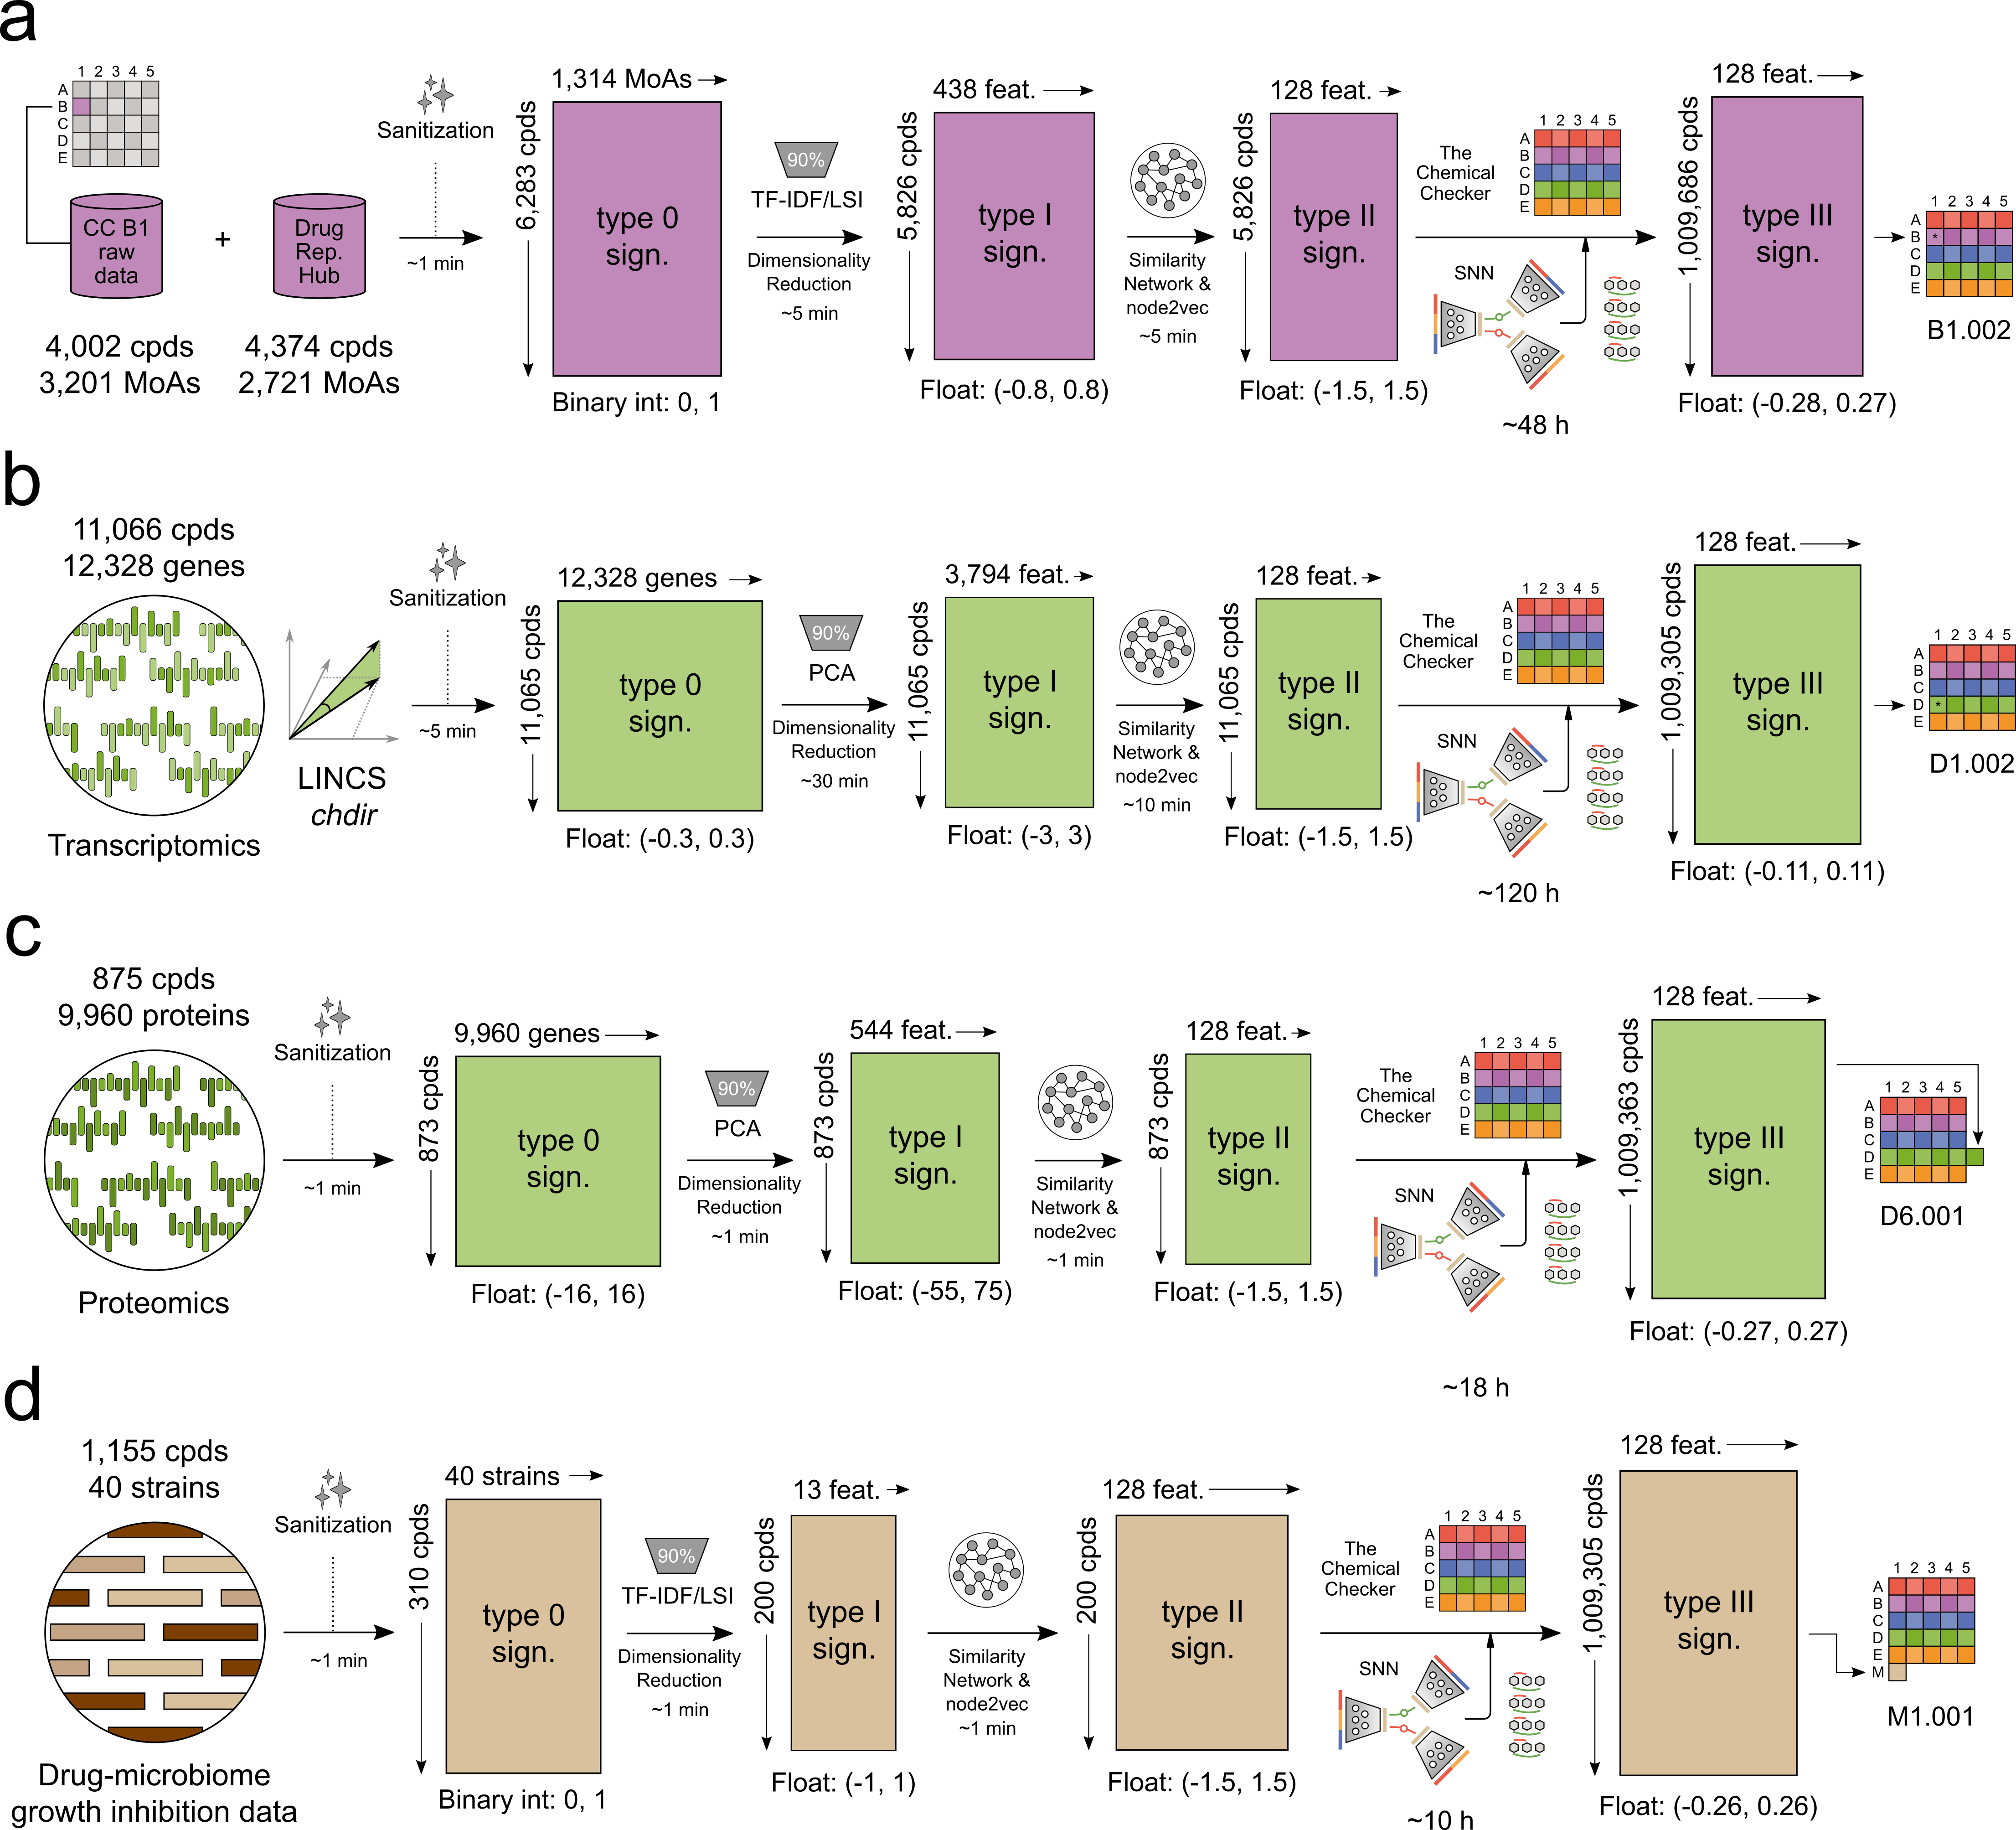
\includegraphics[width=\linewidth]{figures/Protocols/Main/Pipeline_v4.png}
  \caption{
    \textbf{CC Protocols case examples.} 
    \textbf{a)} Extending a preexisting CC space with additional bioactivity data (Task 1: B1.001).
    \textbf{b)} Rebuilding a preexisting CC space with a different strategy of processing the raw data (Task 2: D1.002).
    \textbf{c)} Create a new CC space from a novel data type that fits the current CC universe (i.e. human-derived data. Task 3: D6.001). 
    \textbf{d)} Create a new CC space from a novel data type that does not fit the current CC universe (i.e. measuring compound effects on bacterial species. Task 4: M1.001).
    \rule[0ex]{\textwidth}{0.5pt}
  }
  \label{Protocols_Fig2}
\end{figure}


%%%%%%%%%%%%%%%%%%%%%%%%%%%%
%%%%%%%%%%%%%%%%%%%%%%%%%%%%
%%%%%%%%  D1.002  %%%%%%%%%%
%%%%%%%%%%%%%%%%%%%%%%%%%%%%
%%%%%%%%%%%%%%%%%%%%%%%%%%%%



\phantomsection
\subsubsection{Task 2: Rebuilding a preexisting CC space with a different strategy of processing the raw data (D1.002)}


\paragraph{-- Dataset description --} \leavevmode

Gene expression (GEx) responses after compound perturbation provide a convenient way to connect diseases to drugs. Since the release of the Connectivity Map (CMap) and LINCS resources, compound GEx signatures have allowed the identification of potential treatments for diverse diseases \cite{pauls_identification_2021, sawada_predicting_2018, chen_reversal_2017} and have provided new insights on compounds’ mechanisms of action (MoAs), compounds’ target and sensitivity responses. Given the significant value of these screenings, conscious efforts have been carried out to remove potential sources of noise and inherent biases, unearthing higher and more robust biological signals. Particularly relevant has been the implementation of the Characteristic Direction (chdir) method\cite{clark_characteristic_2014} which, having been tailored in the context of compound perturbation responses, it is not only more suitable for detecting meaningful GEx changes but also provides a means to identify non-robust, noisy profiles. Thus, we re-processed raw LINCS data using the chdir GEx profile protocol, as indicated by the authors. Eventually, we ended up with 11,066 compounds (rows) and 12,328 genes (columns), which significantly enhanced the interpretability compared to the previous processing method. In the next paragraphs we exemplify the rebuilding of the D1 space with this new pre-processing protocol (D1.002). 

\paragraph{-- Signaturization results --}  \leavevmode

After processing the data, we started the rebuilding of the D1 space (D1.002) with 11,066 compounds (rows) and 12,328 genes (columns), while our old processing (D1.001) contained 14,098 compounds and 7,967 CMap features. This reduction in the number of compounds is due to the additional chdir filtering step that accounts for the robustness in the GEx replicates. Now, each compound-gene pair was associated with a numerical value representing the induced gene expression change. After creating the new CC instance and loading the preprocessed bioactivity data, we obtained type 0 signatures for 11,066 compounds against 12,328 genes. It is important to note that, in the generation of type 0 signatures, we set the number of maximally considered features in the sanitization process up to 13k, since the default value is 10k. In addition, we observed that signatures were not redundant and that most values were in the [-0.05, 0.05] range (Fig \ref{Protocols_FigS4}a). Then, we obtained type I signatures for 11,065 compounds with 3,794 dimensions and generated harmonized type II signatures for these 11,065 compounds (Fig \ref{Protocols_FigS4}b, c). Finally, we integrated the D1.002 space with the rest of CC spaces and obtained type III signatures for all 1,009,305 compounds (Fig \ref{Protocols_FigS5}). 

A downstream comparison with the space obtained from our old processing (D1.001) confirmed the overall improved consistency of this new space, as illustrated by the better recapitulation of known drug bioactivity associations, including their MoA and therapeutic (ATC) areas (Fig \ref{Protocols_FigS6}). This exercise highlights the importance not only of the quality of the raw data employed to develop the bioactivity descriptors but also of the preprocessing strategies.

A global picture of the pipeline with detailed steps, numbers and timings is shown in Fig \ref{Protocols_Fig2}b. Diagnosis plots for all signatures are shown in Fig \ref{Protocols_FigS4} and Fig \ref{Protocols_FigS5}.


\phantomsection
\subsubsection{Task 3: Creating a new CC space from a novel data type that fits the current CC universe (D6.001)}

\paragraph{-- Dataset description --} \leavevmode

Deconvoluting the mechanisms of action (MoAs) of bioactive compounds within human cells is fundamental to tailor the eventual therapeutic effects they may exert. To study changes in protein levels induced by the presence of pharmacological agents, Mitchell et al.\cite{mitchell_proteome-wide_2023} screened a collection of 875 small molecule perturbagens in HCT116 cells and derived the so-called ‘proteome fingerprints’ for them, accounting for the changes in protein abundance caused after 24h of treatment and achieving deep proteome coverage (>9,000 quantified proteins). In short, they observed that over half of the quantified proteome changed by at least twofold with at least one compound, and 98\% of the proteins showed a variation of five standard deviations produced by at least one compound. 

Although cell-based assays are indeed included in the CC (e.g. transcriptomics in D1 or sensitivity profiles in D2), proteomics data are not specifically considered. The main purpose of this exercise is to create a new CC space with the proteomics data presented above (namely D6.001) accounting for 875 compounds and 9,960 proteins.  

\paragraph{-- Signaturization results --}  \leavevmode

After creating the new CC instance and loading the preprocessed bioactivity data, we found that 12.5\% of the pairs did not have a reported (log2) fold change measurement (NaNs). We then obtained type 0 signatures for 873 compounds against 9,960 proteins and we observed that signatures were binary and completely non-redundant (Fig \ref{Protocols_FigS7}a). After that, we reduced their dimensionality by generating type I signatures for 873 compounds with 544 features and we then obtained type II signatures for these 873 compounds, at that point already harmonized with the other CC spaces (128 features). Finally, we derived type III signatures for these 873 compounds together with all the CC universe of small molecules, totaling to 1,009,363 signatures (Fig \ref{Protocols_FigS8}). Additionally, when we compared the proteomics signatures to those derived from transcriptomics, we observed that proteomics-based D6.001 type III signatures were able to recapitulate known MoAs at pair with the new D1.002 signatures, and better that the original D1.001 space (Fig \ref{Protocols_FigS9}a, c, e). D6.001 is also better at capturing therapeutic areas (ATC) than the transcriptional spaces, perhaps reflecting protein abundance is a closer proxy for clinical outcomes (Fig \ref{Protocols_FigS9}b, d, f). We also asked if proteomics-derived signatures were able to recapitulate nearest-neighbors in transcriptomics signatures, finding a moderate capacity (AUROC of 0.72 and 0.74 for D1.001 and D1.002, respectively), which indicates a high degree of complementarity between the two bioactivity spaces (Fig \ref{Protocols_FigS9}g, h).

A global picture of the pipeline with detailed steps, numbers and timings is shown in Fig \ref{Protocols_Fig2}c. Diagnosis plots for all signatures are shown in Fig \ref{Protocols_FigS7} and Fig \ref{Protocols_FigS8}. 


\phantomsection
\subsubsection{Task 4: Creating a new CC space from a novel data type that does not fit the current CC universe (M1.001)}


\paragraph{-- Dataset description --} \leavevmode

Non-antibiotic marketed drugs have been recently associated with changes in the composition of the human gut microbiome\cite{weersma_interaction_2020}. Such unforeseen activity may explain potential antibiotic-like side effects, might promote antibiotic resistance and may eventually contribute to a significant decrease in microbiome diversity\cite{maier_extensive_2018}. To unravel potential relationships between non-antibiotic drugs and microbes, Maier et al.\cite{maier_extensive_2018} screened a collection of drug-like compounds (including human-targeted drugs, antibiotics, anti-infective compounds and veterinary drugs, among others) against a set of 40 representative gut bacterial strains. Indeed, they observed that 24\% of the drugs having human targets were able to inhibit the growth of at least one gut bacterial strain \textit{in vitro}. We exhaustively processed their data and defined a binary growth inhibition matrix between tested compounds and strains. The novel bioactivity data involved 1,155 compounds (marketed drugs, rows) tested against 40 representative gut bacterial strains (columns). The main purpose of this exercise is to create a new CC space (i.e. M1.001) where the chemical compounds exert their bioactivities on microbial species in the human microbiota.

\paragraph{-- Signaturization results --}  \leavevmode

After creating the new CC instance and loading the preprocessed bioactivity data, we obtained type 0 signatures for 310 compounds against 40 gut bacterial strains. In fact, we found that 769 molecules exhibited null bioactivity profiles and were thus filtered out from the signaturization process (\textit{min\_keys\_abs} parameter). Additionally, 76 compounds were removed due to an excessive proportion of positive features (\textit{max\_keys\_freq} parameter). After that, we obtained type I signatures for 200 compounds against 13 features, significantly reducing the number of dimensions of the data (Fig \ref{Protocols_FigS10}). We then generated type II signatures for these molecules, harmonizing the number of features to all the other spaces in the CC (128 features). Finally, we derived type III signatures for these 200 compounds and for all the remaining molecules in the CC universe (1,009,305 molecules, in total). 

The construction of the M1.001 space was challenging since, despite the apparent initially high number of compounds and features (i.e. microbial species), the final number or compound-microbe relationships was quite limited. Nevertheless, we still observed a remarkable capacity of type III signatures to recapitulate known MoAs and ATC for annotated compounds (Fig \ref{Protocols_FigS11}).

A global picture of the pipeline with detailed steps, numbers and timings is shown in Fig \ref{Protocols_Fig2}d. Diagnosis plots for all signatures are shown in Fig \ref{Protocols_FigS10} and Fig \ref{Protocols_FigS11}.

